%----------------------------------------------------------------------------------------
% Trapezoidal rule to approximate area under a function
%----------------------------------------------------------------------------------------

\section{Trapezoidal rule to approximate area under $f(x)=x^4$ in OpenMP}

\subsection{Compile and run the template code with a single thread, for $a=0$,
$b=1$, $n=2^{30}$, and thus verify that the serial version is correct, also
checking the calculation by hand.}

\begin{figure}[ht]
	\centering
	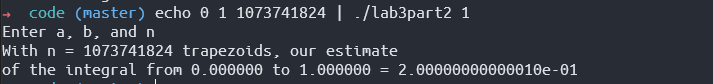
\includegraphics[width=\textwidth]{graphics/P2_a_terminal_output.PNG}
	\caption{Terminal output for $a=0$, $b=1$, $n=2^{30}$}
	\label{fig:P2_a}
\end{figure}


The following shows the calculation to compute by hand:
\vspace{1cm}
\begin{align*}
	\text{Area} &= \int_{0}^{1} x^4 \\
				&= \left[ \frac{x^5}{5} \right]^{1}_{0} \\
				&= \frac{1^5}{5} - \frac{0^5}{5} \\
				&= 0.2
\end{align*}

The computed integral using the trapezoidal rule equals to the answer worked out
by hand analytically using calculus (There is a negligible difference due to base
two floating-point numbers limitation to represent 1/20)

\subsection{Parallelize the code for multi-threaded execution by adding to 
it as few OpenMP directives as possible.}

\vspace{0.5cm}
\lstinputlisting[
	style=CStyle,
	firstline=63, % First line of code
	lastline=85, % Lastl ine of code
	caption=Parallizing the code for multi-threaded execution (line 56-78 in lab3part2.c), % Caption above the listing
	label=lst:lab3part2a, % Label for referencing this listing
	frame=single, % Frame around the code listing
	showstringspaces=false, % Don't put marks in string spaces
	numbers=left, % Line numbers on left
	numberstyle=\normalsize % Line numbers styling
	]{../code/lab3part2.c}
	
\subsubsection{At what points in the code new threads are forked and joined?}
Parallization occurs within the for loop though the use of OpenMP \emph{parallel 
for}. The \emph{for} pragma do not create a team of threads; instead they take
the team of threads that is active, and divide the loop iterations over them.

Since no threads were created prior to the pragma at line 17 in \cref{lst:lab3part2a},
this will be the point which new threads are forked. Threads are then joined
once the team of threads complete the iterations.

\subsubsection{Which parts of code is executed by which threads?}

The main thread will execute all the code outside the parallel region, I.E.
outside the for loop at line 17 in \cref{lst:lab3part2a}. Within the for loop,
OpenMP will take the team of thread that is active, and divide the loop iterations
over them which include the main thread, and any slaves thread.

\subsubsection{Where barriers if any in terms of thread synchronization would be
encountered, and hence how the code achieves parallelization?}

OpenMP creates a critical section and the values stored in  the private variable/s
(in this case it is the \emph{approx} variable) are reduced in the critical section.
This is synchronization that needs to happen to avoid race conditions between threads.

\subsection{Add timing statement to verify that the parallel solution runs faster
than the serial version. Tabulates the speedup and efficiency for 1, 2, 4, 8, threads.}

\begin{center}
\begin{tabular}{|| c | c | c | c ||}
	\hline
	Threads & Time (s) & Speedup & Efficiency (\%) \\ [0.5ex]
	\hline 
	1 & 3.439 & N/A & 100 \\
	2 & 1.920 & 1.791 & 89.557 \\
	4 & 1.252 & 2.747 & 68.67 \\
	8 & 0.754 & 4.561 & 57.013 \\
	\hline
\end{tabular}
\end{center}

\subsubsection{Do the result match the expectation? Why?}

As expected, the more threads will decrease the execution time, however, there
is a diminishing return such that the gain in speed from an increase in thread
diminishes as the thread number increase.

This is due to Amdahl's Law, which effectively state that their is an upper bound
in the speedup regardless the number of threads available unless virtually all of 
a serial program is parallelized. Since only the \emph{for} loop to compute 
the trapezoidal area is parallelized - 
the speed of the program is going to be very much bounded by the serial execution
of the non-parallel portion. 


\subsubsection{Explain why the output differs slightly from run to run for mulitple
thread?}

\begin{figure}[ht]
	\centering
	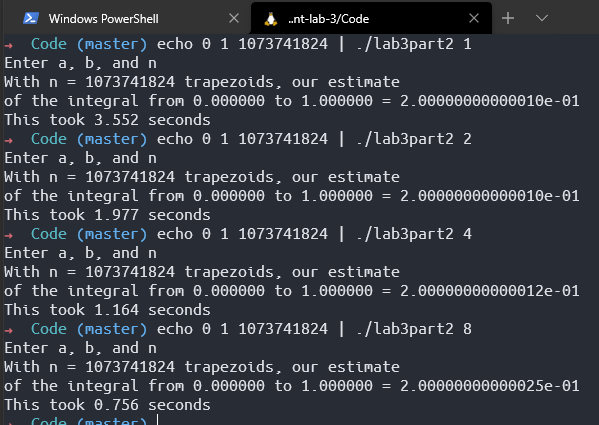
\includegraphics[width=\textwidth]{graphics/P2_c_terminal_output.PNG}
	\caption{Terminal output of execution for varying number of threads}
	\label{fig:lab3part2b}
\end{figure}

As seen in \cref{fig:lab3part2b}, the output differ slightly from run to run. 
The hypothesis is that the reduction is more accurate for higher thread count
due to the fact there is less floating-point precision loss because each thread
is approximating a smaller share of the area. In other words, for an integrand
of $\left[1, 0\right]$, a thread count of two will mean that each thread gets
50\% of the bound, whereas a thread count of 4 means each thread gets 25\% share
of the bound. A smaller bound would mean that there is less floating-point
precision loss as the reduction function is applied.


